\section{Rumus Metode Regresi Linear Berganda}

Analisis regresi linier berganda adalah hubungan secara linear antara dua atau lebih variabel independen (X1, X2) dengan variabel dependen (Y). Analisis ini untuk mengetahui arah hubungan antara variabel independen dengan variabel dependen apakah masing-masing variabel independen berhubungan positif atau negatif dan untuk memprediksi nilai dari variabel dependen apabila nilai variabel independen mengalami kenaikan atau penurunan. Data yang digunakan biasanya berskala interval atau rasio.\citep{smadi2012least}
                        Persamaan regresi linear berganda sebagai berikut:

Y’ = a + b1X1+ b2X2+…..+ bnXn

Keterangan:
Y’                    =   Variabel dependen (nilai yang diprediksikan)
X1 dan X2      =   Variabel independen
a                      =   Konstanta (nilai Y’ apabila X1, X2…..Xn = 0)
b                            =    Koefisien regresi (nilai peningkatan ataupun penurunan)

\newpage \section{Contoh soal Cara Kerja Metode Regresi Linear}
\subsection{Contoh soal 1}
\par Di contoh soal pertama ini penulisa mengambil permasalahan dari kasus di PT Pertamina Gas. Pada kasus di penelitian ini penulis melakukan prediksi \textit{reveniew} dari 5 wilayah milik PT Pertamina Gas. Dan dari setiap wilayah tersebut ada \textit{shipper}(sumber) dan \textit{offtaker}(konsumen)
	Y adalah variabel terikat yang diramalkan (shipper), X adalah variabel bebas. nilai x1(offtaker sinngle) nilai x2 (nilai offtaker multi)\citep{hijriani2017implementasi}
Berikut ini adalah Langkah-langkah dalam melakukan prediksi Regresi Linear Berganda:\citep{analisisrls}
\begin{enumerate}
    \item 	Tentukan nilai a dan b dengan menggunakan SPSS dari 5 wilayah pada PT Pertamina Gas yang di ambil dari data total shipper dan offtaker dari bulan sebelumnya.
     \vspace{9cm}
  \begin{table}[]
  \captionsetup{singlelinecheck=off}
  \caption{\textbf{Eastern Java Area}}
\begin{tabular}{|c|c|c|c|}
\hline
Minggu & Shipper & Single & Multi \\ \hline
1      & 965     & 15     & 308   \\ \hline
2      & 910     & 34     & 616   \\ \hline
3      & 944     & 27     & 616   \\ \hline
4      & 932     & 26     & 637   \\ \hline
5      & 267     & 10     & 183   \\ \hline
\end{tabular}
\end{table}
\newpage \begin{lstlisting}
a= Y-b1X1-b2X2      
a= 325.069
\end{lstlisting}
\begin{figure}[!htbp]
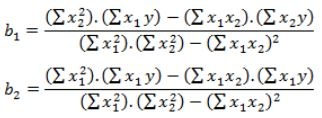
\includegraphics[scale=0.6]{chapters/figures/b1b2.JPG}
    \label{Figure4}
\end{figure}
\begin{lstlisting}
b1= -4.545
b2= 1.23
Rumus:
Y= a+b1X1+b2X2
Y= 325.069+(-4.545x1)+1.23X2
\end{lstlisting}
\vspace{6cm}
\begin{table}[]
  \captionsetup{singlelinecheck=off}
  \caption{\textbf{Kalimantan Area}}
\begin{tabular}{|c|c|c|c|}
\hline
Minggu & Shipper & Single & Multi \\ \hline
1      & 560     & 21     & 378   \\ \hline
2      & 630     & 7     & 378   \\ \hline
3      & 560     & 21     & 378   \\ \hline
4      & 560     & 21     & 378   \\ \hline
5      & 180     & 2     & 108   \\ \hline
\end{tabular}
\end{table}
\newpage \begin{lstlisting}
a= Y-b1X1-b2X2      
a= -0.00000000000014
\end{lstlisting}
\begin{figure}[!htbp]
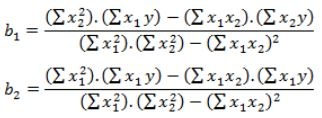
\includegraphics[scale=0.6]{chapters/figures/b1b2.JPG}
    \label{Figure4}
\end{figure}
\begin{lstlisting}
b1= -5
b2= 1.759
Rumus:
Y= a+b1X1+b2X2
Y= -0.00000000000014+(-5x1)+1.759X2
\end{lstlisting}
\vspace{6cm}
\begin{table}[]
  \captionsetup{singlelinecheck=off}
  \caption{\textbf{Northem Sumatra Area}}
\begin{tabular}{|c|c|c|c|}
\hline
Minggu & Shipper & Single & Multi \\ \hline
1      & 597     & 20     & 444   \\ \hline
2      & 646     & 70     & 378   \\ \hline
3      & 737     & 62.01     & 386   \\ \hline
4      & 700     & 70     & 386   \\ \hline
5      & 200     & 20     & 108   \\ \hline
\end{tabular}
\end{table}
\newpage \begin{lstlisting}
a= Y-b1X1-b2X2      
a= 3.319
\end{lstlisting}
\begin{figure}[!htbp]
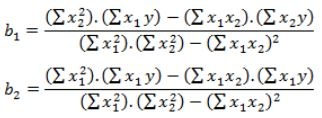
\includegraphics[scale=0.6]{chapters/figures/b1b2.JPG}
    \label{Figure4}
\end{figure}
\begin{lstlisting}
b1= 3.342
b2= 1.207
Rumus:
Y= a+b1X1+b2X2
Y= 3.319+3.342x1+1.207X2
\end{lstlisting}
\vspace{6cm}
\begin{table}[]
  \captionsetup{singlelinecheck=off}
  \caption{\textbf{Southern Sumatra Area}}
\begin{tabular}{|c|c|c|c|}
\hline
Minggu & Shipper & Single & Multi \\ \hline
1      & 640.43     & 9     & 378   \\ \hline
2      & 665.96     & 8     & 378   \\ \hline
3      & 630     & 13     & 378   \\ \hline
4      & 630     & 9     & 378   \\ \hline
5      & 180     & 2     & 108   \\ \hline
\end{tabular}
\end{table}
\newpage \begin{lstlisting}
a= Y-b1X1-b2X2      
a= -9.915
\end{lstlisting}
\begin{figure}[!htbp]
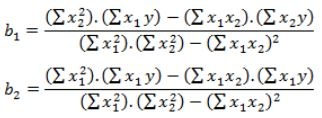
\includegraphics[scale=0.6]{chapters/figures/b1b2.JPG}
    \label{Figure4}
\end{figure}
\begin{lstlisting}
b1= -4.797
b2= 1.847
Rumus:
Y= a+b1X1+b2X2
Y= -9.915+(-4.797x1)+1.847X2
\end{lstlisting}
\vspace{6cm}
\begin{table}[]
  \captionsetup{singlelinecheck=off}
  \caption{\textbf{Western Java Area}}
\begin{tabular}{|c|c|c|c|}
\hline
Minggu & Shipper & Single & Multi \\ \hline
1      & 630     & 14    & 315   \\ \hline
2      & 700     & 14    & 313   \\ \hline
3      & 700     & 14     & 308   \\ \hline
4      & 700     & 14     & 353   \\ \hline
5      & 200     & 4     & 133   \\ \hline
\end{tabular}
\end{table}
\newpage \begin{lstlisting}
a= Y-b1X1-b2X2      
a= -15.599
\end{lstlisting}
\begin{figure}[!htbp]
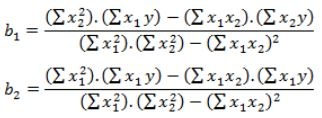
\includegraphics[scale=0.6]{chapters/figures/b1b2.JPG}
    \label{Figure4}
\end{figure}
\begin{lstlisting}
b1= 40.786
b2= 0.394
Rumus:
Y= a+b1X1+b2X2
Y= -15.599+40.786x1+0.394X2
\end{lstlisting}
\newpage \item Setelah itu masukkan ke rumus untuk memprediksi nilai Y(shipper). Y= a+b1X1+b2X2
\item Setelah nilai Y di temukan di kurangkan kembali dengan nilai total perminggu offtaker single dan multi untuk mengetahui sisa shipper.
\item Setelah di temukan nilai total pendapatan perminggu kemudian di jumlahkan untuk mengetahui total pendapatan perbulan
\item Untuk mengetahui reveniew nya total perbulan di akumulasikan ke dollar (perkalian 1MSCF= 4 US dollar).

\end{enumerate}
 \par Berikut adalah hasil perhitungan regresi dan prediksi dalam kalkulasi \$ di bulan berikutnya:
\begin{figure}[!htbp]
    \centering
    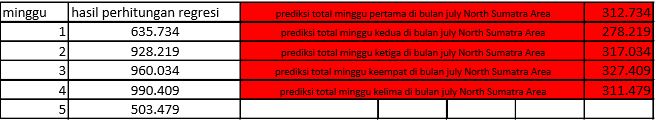
\includegraphics[scale=0.7]{chapters/figures/11.JPG}
\end{figure}
\begin{figure}[!htbp]
    \centering
    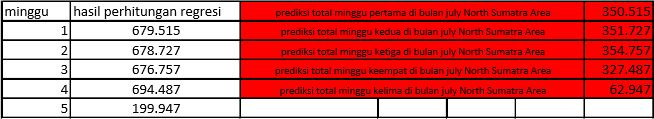
\includegraphics[scale=0.7]{chapters/figures/22.JPG}
\end{figure}
\begin{figure}[!htbp]
    \centering
    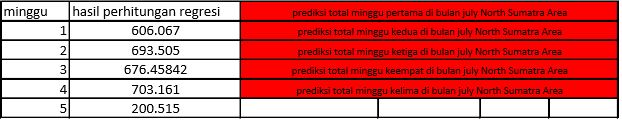
\includegraphics[scale=0.7]{chapters/figures/33.JPG}
\end{figure}
\begin{figure}[!htbp]
    \centering
    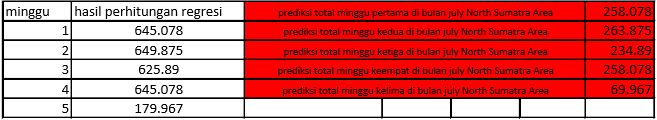
\includegraphics[scale=0.7]{chapters/figures/44.JPG}
\end{figure}
\begin{figure}[!htbp]
    \centering
    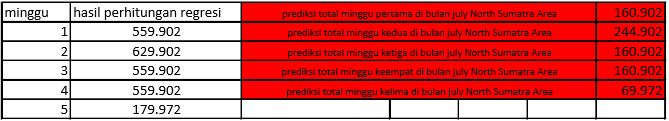
\includegraphics[scale=0.7]{chapters/figures/55.JPG}
\end{figure}
\newpage  \subsection{Contoh soal 2}
\par Kita mengambil contoh kasus pada uji normalitas, yaitu sebagai berikut: Seorang mahasiswa bernama Bambang melakukan penelitian tentang faktor-faktor yang mempengaruhi harga saham pada perusahaan di BEJ.\citep{priyatno2014spss} Bambang dalam penelitiannya ingin mengetahui hubungan antara rasio keuangan PER dan ROI terhadap harga saham. Dengan ini Bambang menganalisis dengan bantuan program SPSS dengan alat analisis regresi linear berganda. Dari uraian di atas maka didapat variabel dependen (Y) adalah harga saham, sedangkan variabel independen (X1 dan X2) adalah PER dan ROI.
Data-data yang di dapat berupa data rasio dan ditabulasikan sebagai berikut: \begin{figure}[!htbp]
    \centering
    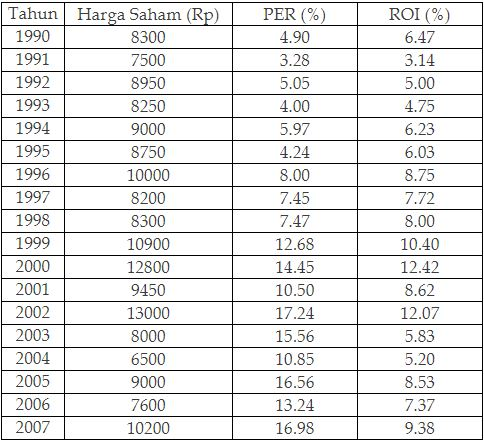
\includegraphics[scale=0.7]{chapters/figures/cs.JPG}
    \caption{Tabulasi Data (Data Fiktif)}
\end{figure}
\newpage \par Langkah berikutnya sama dengan langkah di contoh soal 1. Mencari nilai a dan b nya. \begin{lstlisting}
a= Y-b1X1-b2X2      
a= 4662.491
\end{lstlisting}
\begin{figure}[!htbp]
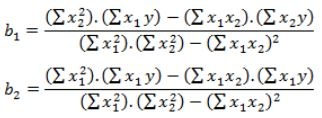
\includegraphics[scale=0.6]{chapters/figures/b1b2.JPG}
    \label{Figure4}
\end{figure}
\begin{lstlisting}
b1= -74.482
b2= 692.107
\end{lstlisting}
Setelah variabel a dan b di temukan maka di masukkan ke dalam rumus seperti berikut: 
Persamaan regresinya sebagai berikut:
\begin{lstlisting}
Y’ = a + b1X1+ b2X2
Y’ =  4662,491 + (-74,482)X1 + 692,107X2
Y’ =  4662,491 - 74,482X1 + 692,107X2
\end{lstlisting}
Keterangan:
\begin{lstlisting}
Y’        = Harga saham yang diprediksi (Rp)
a          = konstanta
b1,b2    = koefisien regresi
X1        = PER (\%)
X2        = ROI (\%)
\end{lstlisting}
\par Langkah berikutnya adalah memasukkan nilai x1(PER (\%)) dan x2(ROI (\%)) ke dalam rumus, sehingga di temukan hasil prediksi sebagai berikut:
\begin{figure}[!htbp]
    \centering
    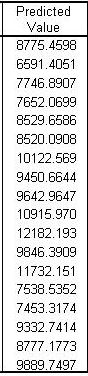
\includegraphics[scale=0.6]{chapters/figures/cs3.JPG}
    \caption{Hasil Perhitungan Prediksi}
\end{figure}
\newpage \subsection{Contoh soal 3}
\par Di contoh soal 3 ini kita akan menghitung data pengeluaran 10 rumah tangga, untuk pembelian barang tahan lama per minggu(Y), pendapatan per minggu (X1), dan jumlah anggota keluarga (X2).
\par Berikut adalah data mentahan nya:
\begin{figure}[!htbp]
    \centering
    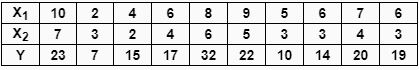
\includegraphics[scale=0.7]{chapters/figures/css.JPG}
    \caption{Data mentahan}
\end{figure}


